% THIS IS SIGPROC-SP.TEX - VERSION 3.1
% WORKS WITH V3.2SP OF ACM_PROC_ARTICLE-SP.CLS
% APRIL 2009
%
% It is an example file showing how to use the 'acm_proc_article-sp.cls' V3.2SP
% LaTeX2e document class file for Conference Proceedings submissions.
% ----------------------------------------------------------------------------------------------------------------
% This .tex file (and associated .cls V3.2SP) *DOES NOT* produce:
%       1) The Permission Statement
%       2) The Conference (location) Info information
%       3) The Copyright Line with ACM data
%       4) Page numbering
% ---------------------------------------------------------------------------------------------------------------
% It is an example which *does* use the .bib file (from which the .bbl file
% is produced).
% REMEMBER HOWEVER: After having produced the .bbl file,
% and prior to final submission,
% you need to 'insert'  your .bbl file into your source .tex file so as to provide
% ONE 'self-contained' source file.
%
% Questions regarding SIGS should be sent to
% Adrienne Griscti ---> griscti@acm.org
%
% Questions/suggestions regarding the guidelines, .tex and .cls files, etc. to
% Gerald Murray ---> murray@hq.acm.org
%
% For tracking purposes - this is V3.1SP - APRIL 2009

\documentclass{acm_proc_article-sp}

\begin{document}

\title{Predicting the Feasibility of Unseen Test Cases}
\numberofauthors{2}
\author{
% 1st. author
\alignauthor
Bryan Robbins\\
       \affaddr{University of Maryland - College Park}\\
       \affaddr{Department of Computer Science}\\
       \affaddr{4115 AV Williams Building}\\
       \affaddr{College Park, MD 20742}\\
       \email{brobbins@cs.umd.edu}
% 2nd. author
\alignauthor
Atif Memon\\
       \affaddr{University of Maryland - College Park}\\
       \affaddr{Department of Computer Science}\\
       \affaddr{4115 AV Williams Building}\\
       \affaddr{College Park, MD 20742}\\
       \email{atif@cs.umd.edu}
}
\maketitle
\begin{abstract}
This is the abstract.
\end{abstract}

\category{D.2.5}{Software Engineering}{Testing and Debugging}
\terms{Experimentation, Verification}
\keywords{Software testing, model-based testing, test automation}

\section{Introduction}
Model-based software testing excels at the generation of short test cases. Often,
the collective group of test cases (called the test suite) provides a guarantee
of coverage. Consider various existing work by Memon et al., which generates test
cases for event-driven systems such as those driven by Graphical User Interfaces
(GUIs). Their sequence length coverage generation technique experiences an
exponential growth of possible test cases as longer sequence lengths are considered. This
growth often leads to a practical limit of considering only coverage of sequences 
of length 2 or 3 when generating test suites. Other research suggests that longer
test cases can more efficiently and more effectively find bugs than shorter test
cases.

In this paper, we lay the groundwork for constructing longer test cases from the shorter
test cases typical of model-based testing techniques. We explore whether shorter test cases
can be combined in interesting ways to produce longer test cases while still preserving
desired characteristics. As a first step, we consider the preservation of test case
feasibility. More precisely, we explore whether the execution results of model-based test
cases can be used to predict the feasibility of potential test case combinations. We believe
that this work can later be extended to the prediction of additional test suite properties,
and eventually to generalized reduction techniques for model-based test suites; but
we do not explore those extensions in this work.



\section{The {\secit Body} of The Paper}

\subsection{Tables}
Because tables cannot be split across pages, the best
placement for them is typically the top of the page
nearest their initial cite.  To
ensure this proper ``floating'' placement of tables, use the
environment \textbf{table} to enclose the table's contents and
the table caption.  The contents of the table itself must go
in the \textbf{tabular} environment, to
be aligned properly in rows and columns, with the desired
horizontal and vertical rules.  Again, detailed instructions
on \textbf{tabular} material
is found in the \textit{\LaTeX\ User's Guide}.

Immediately following this sentence is the point at which
Table 1 is included in the input file; compare the
placement of the table here with the table in the printed
dvi output of this document.

\begin{table}
\centering
\caption{Frequency of Special Characters}
\begin{tabular}{|c|c|l|} \hline
Non-English or Math&Frequency&Comments\\ \hline
\O & 1 in 1,000& For Swedish names\\ \hline
$\pi$ & 1 in 5& Common in math\\ \hline
\$ & 4 in 5 & Used in business\\ \hline
$\Psi^2_1$ & 1 in 40,000& Unexplained usage\\
\hline\end{tabular}
\end{table}

To set a wider table, which takes up the whole width of
the page's live area, use the environment
\textbf{table*} to enclose the table's contents and
the table caption.  As with a single-column table, this wide
table will ``float" to a location deemed more desirable.
Immediately following this sentence is the point at which
Table 2 is included in the input file; again, it is
instructive to compare the placement of the
table here with the table in the printed dvi
output of this document.


\begin{table*}
\centering
\caption{Some Typical Commands}
\begin{tabular}{|c|c|l|} \hline
Command&A Number&Comments\\ \hline
\texttt{{\char'134}alignauthor} & 100& Author alignment\\ \hline
\texttt{{\char'134}numberofauthors}& 200& Author enumeration\\ \hline
\texttt{{\char'134}table}& 300 & For tables\\ \hline
\texttt{{\char'134}table*}& 400& For wider tables\\ \hline\end{tabular}
\end{table*}
% end the environment with {table*}, NOTE not {table}!

\subsection{Figures}
Like tables, figures cannot be split across pages; the
best placement for them
is typically the top or the bottom of the page nearest
their initial cite.  To ensure this proper ``floating'' placement
of figures, use the environment
\textbf{figure} to enclose the figure and its caption.

This sample document contains examples of \textbf{.eps}
and \textbf{.ps} files to be displayable with \LaTeX.  More
details on each of these is found in the \textit{Author's Guide}.

\begin{figure}
\centering
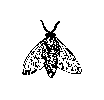
\epsfig{file=images/fly.eps}
\caption{A sample black and white graphic (.eps format).}
\end{figure}

\begin{figure}
\centering
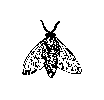
\epsfig{file=images/fly.eps, height=1in, width=1in}
\caption{A sample black and white graphic (.eps format)
that has been resized with the \texttt{epsfig} command.}
\end{figure}


As was the case with tables, you may want a figure
that spans two columns.  To do this, and still to
ensure proper ``floating'' placement of tables, use the environment
\textbf{figure*} to enclose the figure and its caption.

Note that either {\textbf{.ps}} or {\textbf{.eps}} formats are
used; use
the \texttt{{\char'134}epsfig} or \texttt{{\char'134}psfig}
commands as appropriate for the different file types.

\subsection{Theorem-like Constructs}
Other common constructs that may occur in your article are
the forms for logical constructs like theorems, axioms,
corollaries and proofs.  There are
two forms, one produced by the
command \texttt{{\char'134}newtheorem} and the
other by the command \texttt{{\char'134}newdef}; perhaps
the clearest and easiest way to distinguish them is
to compare the two in the output of this sample document:

This uses the \textbf{theorem} environment, created by
the\linebreak\texttt{{\char'134}newtheorem} command:
\newtheorem{theorem}{Theorem}
\begin{theorem}
Let $f$ be continuous on $[a,b]$.  If $G$ is
an antiderivative for $f$ on $[a,b]$, then
\begin{displaymath}\int^b_af(t)dt = G(b) - G(a).\end{displaymath}
\end{theorem}

The other uses the \textbf{definition} environment, created
by the \texttt{{\char'134}newdef} command:
\newdef{definition}{Definition}
\begin{definition}
If $z$ is irrational, then by $e^z$ we mean the
unique number which has
logarithm $z$: \begin{displaymath}{\log e^z = z}\end{displaymath}
\end{definition}

\begin{figure}
\centering

\psfig{file=images/rosette.pdf, height=1in, width=1in,}
\caption{A sample black and white graphic (.ps format) that has
been resized with the \texttt{psfig} command.}
\end{figure}

Two lists of constructs that use one of these
forms is given in the
\textit{Author's  Guidelines}.

\begin{figure*}
\centering
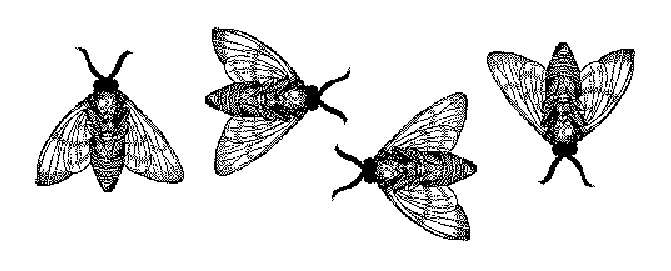
\epsfig{file=images/flies.eps}
\caption{A sample black and white graphic (.eps format)
that needs to span two columns of text.}
\end{figure*}
and don't forget to end the environment with
{figure*}, not {figure}!
 
There is one other similar construct environment, which is
already set up
for you; i.e. you must \textit{not} use
a \texttt{{\char'134}newdef} command to
create it: the \textbf{proof} environment.  Here
is a example of its use:
\begin{proof}
Suppose on the contrary there exists a real number $L$ such that
\begin{displaymath}
\lim_{x\rightarrow\infty} \frac{f(x)}{g(x)} = L.
\end{displaymath}
Then
\begin{displaymath}
l=\lim_{x\rightarrow c} f(x)
= \lim_{x\rightarrow c}
\left[ g{x} \cdot \frac{f(x)}{g(x)} \right ]
= \lim_{x\rightarrow c} g(x) \cdot \lim_{x\rightarrow c}
\frac{f(x)}{g(x)} = 0\cdot L = 0,
\end{displaymath}
which contradicts our assumption that $l\neq 0$.
\end{proof}

Complete rules about using these environments and using the
two different creation commands are in the
\textit{Author's Guide}; please consult it for more
detailed instructions.  If you need to use another construct,
not listed therein, which you want to have the same
formatting as the Theorem
or the Definition\cite{salas:calculus} shown above,
use the \texttt{{\char'134}newtheorem} or the
\texttt{{\char'134}newdef} command,
respectively, to create it.

\subsection*{A {\secit Caveat} for the \TeX\ Expert}
Because you have just been given permission to
use the \texttt{{\char'134}newdef} command to create a
new form, you might think you can
use \TeX's \texttt{{\char'134}def} to create a
new command: \textit{Please refrain from doing this!}
Remember that your \LaTeX\ source code is primarily intended
to create camera-ready copy, but may be converted
to other forms -- e.g. HTML. If you inadvertently omit
some or all of the \texttt{{\char'134}def}s recompilation will
be, to say the least, problematic.

\section{Conclusions}
This is the conclusion.


\bibliographystyle{abbrv}
\bibliography{amalga}
\balancecolumns
\end{document}
